\documentclass{article}

\usepackage{amsmath}
\usepackage{graphicx}
\usepackage{subcaption}
\usepackage{amssymb}
\usepackage{ulem}
\usepackage{enumerate}
\usepackage{pdfpages}
\usepackage{soul}

\DeclareMathOperator{\sech}{sech}
\DeclareMathOperator{\csch}{csch}
\DeclareMathOperator{\arcsec}{arcsec}
\DeclareMathOperator{\arccot}{arcCot}
\DeclareMathOperator{\arccsc}{arcCsc}
\DeclareMathOperator{\arccosh}{arcCosh}
\DeclareMathOperator{\arcsinh}{arcsinh}
\DeclareMathOperator{\arctanh}{arctanh}
\DeclareMathOperator{\arcsech}{arcsech}
\DeclareMathOperator{\arccsch}{arcCsch}
\DeclareMathOperator{\arccoth}{arcCoth} 


\newcommand\longdiv[2]{%
$\strut#1$\kern.25em\smash{\raise.3ex\hbox{$\big)$}}$\mkern-8mu
        \overline{\enspace\strut#2}$}

\title{Calculus Notes}
\date{Fri, 12 Feb. 2021}
\author{Ahmed Gamal Eltokhy}

\begin{document}
\maketitle
\pagenumbering{gobble}
\newpage

\tableofcontents
\newpage

\pagenumbering{arabic}

\part{Calculus II}
\newpage

\section{Vectors}

\subsection{The 3D space}

When you have a constant in 3D, then the graph will have a plane parallel to the base the unit vector is perpendicular to.

e.g. for the equation $x^2+y^2=25, z=-8$ all points will lie in the horizontal plane of $z=-8$. Also, since $x^2+y^2=25$ then the graph will have the region with all points lying on a circle with radius $\sqrt{25}$.

\paragraph{Common Sense Facts:}

If $A(x,y,z)$ and $B(h,k,l)$, then $\vec{AB}$ will be $AB(h-x, k-y, l-z)$.

The length of vectors will be equal to the square root for adding their squared values. e.g. For the vector $\vec{a}<x,y,z>$
\begin{equation*}
	|\vec{a}| = \sqrt{x^2+y^2+z^2}
\end{equation*}

Also, addition, subtraction, scalar multiplication of two vectors algebraically will be just the addition or subtraction or the scalar multiplication of their coordinates.



\subsection{The sphere}

For the sphere with center $C(h,k,l)$ and radius $r$, the equation will be

\begin{equation}
	(x-h)^2 + (y-k)^2 +(z-3)^2 = r^2
\end{equation}

e.g. For the equation $(x+2)^2 + y^2 + (z-3)^2 = 16$ the center of the circle will be $C(-2,0,3)$ and the radius will be $ \sqrt{16} = 4$. Also, a sphere with center the origin will have the equation $x^2+y^2+z^2=r^2$.

\subsection{Vectors addition}

To sum vectors $\vec{u}, \vec{v}$ you will position the vectors as the initial point of $\vec{v}$ is the terminal point of $\vec{u}$. The sum will be the vector from initial point of $\vec{u}$ to the terminal point of $\vec{v}$.

On the same base, and since $-\vec{b}$ will be the same as the vector but in the opposite direction, $\vec{u} - \vec{v}$ will connect the tip of $\vec{v}$ to the tip of $\vec{u}$

\begin{figure}[h!]
	\includegraphics[width=0.7\linewidth]{./vectoraddtion.jpg}
	\caption{Representing vectors addition in two manners.}
\end{figure}

\begin{figure}[h!]
	\includegraphics[width=1\linewidth]{./2021-02-05_09-59.png}
	\caption{An example for calculating vectors by Stewart Calculus.}
\end{figure}	

\paragraph{More example} \

\subparagraph{Question}
Find the unit vectors that are parallel to the tangent line to the parabola $y=x^2$ at the point $(2,4)$

\subparagraph{Solution}
The tangent line will be $ \frac{dy}{dx}(x^2) = 2x = 2(2) = 4$ then the parallel lines to that vector will be the vectors $<1,4>,<-1,-4>$. To get the unit vectors, equalize the magnitude to 1. 

$|<1,4>| = \sqrt{1^2 + 4^2} = \sqrt{17}$. Thus the unit vectors will be $\pm\frac{1}{17}<1,4>$

\newpage

\subsection{Dot Product}

\paragraph{Formulas}

\begin{equation}
	\vec{a} . \vec{b} = |a||b| \cos{\theta} 
\end{equation}
\begin{equation}
	\vec{a} . \vec{b} = (a_1)(b_1) + (a_2)(b_2) + (a_3)(b_3)
\end{equation}

\paragraph{Direction Angles}
They are $\alpha, \beta, \gamma$ in the interval $[0,\pi]$ that a vector $\vec{a}$ makes with positive $x,y,z$ axis. Cosines of these angles must equal 1.

\begin{equation}
	\cos{\alpha} = \frac{\vec{a} . \vec{i}}{|\vec{a}| |\vec{i}|} = \frac{a_1}{|\vec{a}|}
\end{equation}

\begin{equation*}
	\cos{\beta} = \frac{a_2}{|a|} \qquad \cos{\gamma} = \frac{a_3}{|a|}	
\end{equation*}

Squaring the previous equations, we find that

\begin{equation}
	\cos{\alpha}^2 + \cos{\beta}^2 + \cos{\gamma}^2 = 1
\end{equation}

Thus, we can say that direction cosines of $\vec{a}$ are the components of unit vector in the direction of $ \vec{a}$.

\begin{equation}
	\frac{1}{|a|} \vec{a} = <\cos{\alpha} , \cos{\beta} , \cos{\gamma}>
\end{equation}

\noindent\hrulefill 

\newpage

\subsection{Projections}

\subparagraph{Scalar Projections of $ \vec{b}$ onto $ \vec{a}$}
\[comp_a \vec{b} = \frac{ \vec{a} . \vec{b}}{|\vec{a}|}	\]
\subparagraph{Vector Projections of $ \vec{b}$ onto $ \vec{a}$}
\[
	proj_a \vec{b} = 	\frac{ \vec{a} . \vec{b} }{|a|}	 \frac{ \vec{a} }{ |\vec{a}| } = \frac{ \vec{a} . \vec{b} }{| \vec{a} |^2} \vec{a}
\]
\subparagraph{The Orthogonal Vector to the projection}
\[
	orth_a \vec{ b } = \vec{ b } - proj_a \vec{ b }
\]
\begin{figure}[h!]
	\begin{subfigure}{0.5\linewidth}
		\includegraphics[width=0.9\linewidth]{./scalarprojection.png}
		\caption{Scalar Projection of A onto B}
	\end{subfigure} \qquad
	\begin{subfigure}{0.5\linewidth}
		\includegraphics[width=0.9\linewidth]{./vectorprojection.png}
		\caption{Vector Projection of vector $ \vec{b}$ onto $ \vec{a}$ is vector $ \vec{a1}$}
	\end{subfigure}
\end{figure}

\newpage

\subsection{Cross Product}

\subsubsection{Matrix?}
We will use the matrix to track where the unit vectors land after the transformation of some stuff. For instance, in the case of 2x2 Matrix:

\[
	\left [
		\begin{matrix}
			a & b\\
			c & d
		\end{matrix} 
		\right ]
\]

$ a $ and $ c $ track where $ \vec{ i } $ lands. and $ b $ and $ d $ track where $ \vec{ j } $ lands. Thus, any transformation for the grid will be a multiplication of that unit transformation.

\[
	\left [
		\begin{matrix}
			a & b\\
			c & d
		\end{matrix} 
		\right ]
	\left [
		\begin{matrix}
			x \\
			y	
		\end{matrix}
		\right ]
	=
	x \left [
		\begin{matrix}
			a \\ c
		\end{matrix}
		\right]
	+ y \left [
		\begin{matrix}
			b \\ d
		\end{matrix}
		\right]
	= \left [
		\begin{matrix}
			a x + b y \\ c x + d y 
		\end{matrix}
		\right]
\]

Also, the determinant in this manner measure the factor by which the area changes. This area visualized in Figure \ref{3b1b:det1} is what we'll call "cross product". However, it's really not the cross product, it's the magnitude of cross product.

\begin{figure}[h]
	\includegraphics[width=\linewidth]{./2021-02-10_21-22.png}
	\caption{Visualization for the area, aka determinant by 3b1b}
	\label{3b1b:det1}
\end{figure}

\subparagraph{Calculation}
To calculate the "value" aka the determinant or magnitude of the matrix, we follow some simple rules that you can derive from Figure \ref{3b1b:det1}.

\[
	\left [
		\begin{matrix}
			a & b\\c & d
		\end{matrix}
		\right]
	= a d - b c
\]
\[
	\left [
		\begin{matrix}
			\vec{ i } & \vec{ j } & \vec{ k } \\
			a_1 & a_2 & a_3 \\
			b_1 & b_2 & b_3 \\
		\end{matrix}
		\right] = \vec{ i } \left [
		\begin{matrix}
			a_2 & a_3\\
			b_2 & b_3
		\end{matrix}
		\right]
	- \vec{ j } \left [
		\begin{matrix}
			a_1 & a_3\\b_1 & b_3
		\end{matrix}
		\right] + \vec{ k } \left [
		\begin{matrix}
			a_1 & a_2\\b_1 & b_3
		\end{matrix}
		\right]
\]
You will then  calculate using 2D method. You can notice that we "hide" the rows and columns of the value we multiply to and select the remaining.

\subsubsection{The Cross Product}

\subparagraph{Intuition} 

In Figure \ref{3b1b:det1}, we said that the cross product will be the determinant of the two vectors, or the area formed by extending the parallelogram to this vector. The cross product between two vectors will produce a vector perpendicular to the plane formed by the vectors. Only the magnitude of such vector equals the area of the parallelogram formed by extending these two vectors. 
Direction of the cross product in 3D manner can be found using right hand rule. In 2D manner, use the unit vectors method; 
$ \vec{ i } \times \vec{ j } = +1$.

\begin{figure}[h!]
	\includegraphics[width=\linewidth]{./2021-02-10_21-59.png}
	\caption{Cross Product Visualized}
\end{figure}

\subparagraph{TL;DR Formula}
\[
	a\times b = <a_2b_3-a_3b_2,a_3b_1-a_1b_3,a_1b_2-a_2b_1> 
\]
\[
	|a\times b|
	= |a||b| \sin{ \theta } 
\]
\[
	a \parallel b \implies a \times b = 0 
\]
Notice that the cross product is not commutative.
\[
	i \times j = k  \qquad j \times k = i \qquad k \times i = j \qquad j \times i = -k \qquad k \times j = -i \qquad i \times k = -j 
\]

\[
	a . (b \times c) = (a \times b) . c \qquad \qquad a \times (b \times c ) = (a.c)b - (a.b)c 
\]

\newpage

\paragraph{Famous examples}
\subparagraph{The Parallelepiped}
The volume of that figure equals the product between the base and attitude. Thus, we have three vectors $ \vec{ v }, \vec{ u }, \vec{ w } $, the volume can be calculated by getting the cross product of the base (any two of the three vectors). Then, the volume will be the dot product of both the cross product and the third vector, as known as the triple scalar product.
It can also be used to find whether some vectors are coplaner; (that triple product will equal 0)
\begin{equation*}
	( \vec{ v } \times \vec{ u } ) . \vec{ w }
\end{equation*}

However, in the case the question gave you three vectors directly, you can just blot the three vectors on a matrix and solve, the absolute value of the determinant will be the volume.
\begin{equation*}
	Volume = det \left( \left [
		\begin{matrix}
			v_1&v_2&v_3\\u_1&u_2&u_3\\w_1&w_2&w_3
		\end{matrix}
		\right]
	\right)
\end{equation*}

\begin{enumerate}[1.]
	\item For any vectors u and v in V3 and any scalar k, k(u × v) = (ku) × v.
\item For any vectors u and v in V3, (u + v) × v = u × v.
 
\end{enumerate}
\subparagraph{Distance between a line and a point}
\[
	\frac{| \vec{ u } \times \vec{ v }| }{ | \vec{ v } | } 
\]

Where $\vec{ u }$ is some line $ \vec{ AB } $ For instance, and $\vec{ v }$ is the point. \\ 
This equation is visualized as the area of parallelogram divided by the base, as visualized in the cross product above.
\\
\newpage
\subsection{Lines and Planes in 3D}

\subsubsection{Equation of the line}

Firstly remember that any line will be parallel to a unit vector with same direction, and each parallel vector is the scalar multiplication of the vector it is parallel to. Thus, technically any line is just some unit vector that got pushed by some scalar value. To elaborate, let $ \vec{ v } $ is the unit vector parallel to $ \vec{ L } $.
\[
	\therefore \vec{ L } = t . \vec{ v }	\qquad \qquad (1)
\]
In general, the vector equation of the line that's parallel to $ \vec{ v } $ and passes through the point $r_0$, it's equation is
\[
	\vec{ L } = r_0 + t \vec{ v }
\]

Let's let $\vec{ L } = \vec{ P_0P}$ where $ P_0(x_0,y_0,z_0) \& P(x,y,z) \implies \vec{L} = <x-x_0,y-y_0,z-z_0>$. Besides, let $ \vec{ v } = <a,b,c>$. From (1):
\begin{equation*}
	<x-x_0,y-y_0,z-z_0> = t. <a,b,c>  
\end{equation*}
\begin{equation*}
	x-x_0=at \qquad y-y_0=bt \qquad z-z_0=ct \qquad (Parametric Equation)
\end{equation*}
\[
	t= \frac{ x-x_0 }{a} = \frac{ y-y_0 }{b} = \frac{ z-z_0 }{c }   \qquad (Symmetric\ Equation)
\]

\paragraph{Some Important Points}
If one direction is 0, then the line is a plane. If $a=0 \implies x=x_0 $ and the line lies in $x=x_0$ plane, parallel to the yz-plane. 

For the direction vector, you do any scalar multiplication to make the thing easier. You can multiple or divide by some constants for the direction vector \textbf{except} when you're dealing with the distance.

If a / b / c equals zero, you'll write the symmetric equation with z as constant.

\newpage
\subsubsection{Planes}
Remember the normal vector, which is any vector perpendicular to the plane. 
It can be normally got by the cross product of two vectors.
Also, since all normal vectors to a plane will be all parallel, all of them are scalar multiplication of each other. 

Let's play with the same line $ \vec{ P_0P} $ we used in the lines. Also let the normal line to the plane $ \vec{ n } $ where $ \vec{ n } \perp \vec{ P_0P } \implies \vec{ n }\ .\ \vec{ P_0P } = 0$. Actually this is the standard form of a plane. Let's play with that.

The equation of a plane can be got easily using  $\vec{n}$ which is the normal or cross product of the two vectors that form the plane. Then, the equation of the plane will be $ n_1 x + n_2 y + n_3 z = d$
\begin{figure}[h]
	\centering
	\includegraphics[width=0.4\textwidth]{./equationoftheplanevisual.png}
	\caption{Equation of the plane visualization, by Dr. Lotfallah}
	\label{fig:lotfalla_plane_1}
\end{figure}
\[
	\vec{ n }\ .\ \vec{ P_0P } = a(x-x_0) + b(y-y_0) + c(z-z_0) = 0 
\]
\[
	ax+by+cz = ax_0+by_0+cz_0	
\]
Since R.H.S is all constants, they will be denoted by d

\[
	x+by+cz = d
\]



\subsubsection{Remember}

Two planes are $ \parallel $ if their normals are $\parallel$. 
\\
Two planes are $ \perp $ if their normals are $\perp$. \\
Angle between planes = angle between normals.
\\
Scalar multiplication determines parallelism, dot product determine perpendicularism (if it's equal to zero).
\\
Two planes parallel to a line are not necessarily parallel.

\newpage
\subsubsection{Questions}

\begin{enumerate}[1.]
	\item The generic question will provide two points, P and Q for instance, where you will get $ \vec{ v } = \vec{ PQ } $. Then, you'll use a point to solve. For points $ P(-1,-2,-\frac{1}{2}), Q(1,\frac{3}{2}, -3	)$
		\[
			\vec{ v } = \vec{ PQ } = <2, \frac{7}{2}, -\frac{5}{2}> .\ 2 =\  <4,7,-5>
		\]
		By using the point $P$
		\[
			\therefore \quad x = -1+4t \quad y=-2+7t \quad z=-\frac{1}{2}-5t
		\]
		\subparagraph{Also}
		\begin{enumerate}[a.]
			\item  	You can reverse-engineer the previous equation to get the original point by plugging $t=0$.
			\item Or find  the unit vector by getting the coefficients of the t, but make sure that it's only 1 x / y / z.
			\item  You can easily convert to the symmetric form by solving each of the equations to t.
		\end{enumerate}
	\item The second generic question will be whether two lines are intersecting and their intersection point. Firstly, you will make sure they are not parallel by the normal scalar multiplication check. Then, you will equalize each of the parametric equation of the two lines, since the intersection will occur at $x_1=x_2, y_1=y_2, z_1=z_2$. Then, solve for t.
		\[
			L_1 : x_1=1-2t_1,\ y_1 = -1-3t_1,\ z_1=-2+t_1
		\]
		\[
			L_2: x_2=-3+t_2,\ y_2=-2+2t_2,\ z_2=3-t_2
		\]
		\[
			x:\ 1-2t_1 = -3+t_2 \qquad y:\ -1-3t_1=-2+2t_2 \qquad z:\ -2+t_1 = 3-t_2 
		\]
		Solving two equations together.
		\[1-2t_1=-3+t_2 \qquad	\qquad -2+t_1=3-t_2\]
		\[
			-1-t_1=0 \implies t_1=-1,\ t_2=6
		\]

		Then, you will equalize the values you got to the equations in x, y, and z.
		\[
			x:\ 3=3 \qquad y:\ 2 \neq  10 \qquad z:\ -3=-3
		\]
		Thus, since the three equations did not hold with $ t_1, t_2 $ values. Then, the two lines do not intersect. You can think of that as two planes flying at separate times; while they are not parallel, then do not intersect. This line is called \textbf{skew lines}.  

		If $t_1=t_2$ in the last equalization, the point where the intersection happens is simply values of $ <x,y,z> $ 

	\item Another similar question to the previous is asking where a line intersects a plane. Just put the equations of $x,y,z$ in the equation of the plane given, and solve for $t$. Then you'll have the points. 

	\item The generic question will give you two vectors where you will get the normal vector, then you will use any point to get the equation for the plane. So, using a vector and a point will get you the equation of the plane or the line; normal vector in case of plane, and the unit vector parallel to the line in the latter.

	\item \textbf{Find equation for line of intersection} \[
			P_1:\ 2x-3y+4z=3 \qquad \qquad P_2:\ x+4y-2z=7
		\]
		For this question you will need to get the normals of the planes first.
		\[
			n_1=<2,-3,4> \qquad \qquad n_2=<1,4,-2>
		\]
		Then we will need a point, direction vector of the line of intersection. The intuition behind the answer is that the line of intersection will be parallel to the vector which is mutually orthogonal to the two normal to the planes, as shown in \ref{fig:-vectorsnormaltotheplanes-png}.

		\begin{figure}[h!] 
			\centering
			\includegraphics[width=0.4\textwidth]{./vectorsnormaltotheplanes.png}
			\caption{Intersection Line}
			\label{fig:-vectorsnormaltotheplanes-png}
		\end{figure}

		Then, we just get the cross product to figure out $\vec{v}$. 
		\[
			\vec{ n_1 } \times \vec{ n_2 } = <-10,8,11> \qquad \qquad (Direction)
		\]\\\\
		Now, we need a point on the intersection line since we figured the direction. 
		Let's let any variable equal zero and solve for the rest, I'll let $y=0$. 
		\[
			2x+4z=3 \qquad \qquad
			(x-2z=7)2 	
		\]
		\[
			\therefore x = \frac{17}{4} \qquad y = 0 \qquad z = -\frac{11}{8} \qquad (Point)
		\]
		Now, we're done! Let's just put everything in the equation of the line.
		\[
			x = -10t+\frac{17}{4} \qquad y=8t \qquad z= 11t-\frac{11}{8}
		\]
	\item \textbf{Distance between a point and a plane}
		The distance, as viewed in Figure \ref{fig:scapingdistance_1}, will be just the projection of the vector $ \vec{ P_0P_1 } $ denoted by $ \vec{ b } $ onto the normal to the plane. 
		\begin{figure}[h!]
			\centering
			\includegraphics[width=\textwidth]{./componenttogetthedistancevectorplane.png}
			\caption{Scraping to visualize.}
			\label{fig:scapingdistance_1}
		\end{figure}	

		As proved in the dot product 

		\[
			D = Comp_{ \vec{ n } } \vec{ b } 			= \frac{ \vec{ n } . \vec{ b } }{ | \vec{ n }| } = | \vec{ b } | \cos{ \theta } 
		\]
		\\ 
		We can play with the previous formulas. To get $D$ from $P_1(x_1,y_1,z_1)$ to the plane $ax_0+by_0+cz_0+d=0$.
		\[
			D = \frac{ <x_1-x_0, y_1-y_0, z_1-z_0>\ .\ <a,b,c> }{ \sqrt{a^2+b^2+c^2}}=  \frac{ |(ax_1+by_1+cz_1)-(ax+by+cz)| }{ \sqrt{a^2+b^2+c^2} }
		\]
		\[
			d = ax+by+cz \qquad	\therefore D = \frac{ |ax_1+by_1+cz_1-d| }{ \sqrt{a^2+b^2+c^2} }
		\]
		\\

	\item \textbf{Distance between two planes}
		\[
			P_1:5y=2+2x+z \qquad \qquad P_2:4x+2z=7+10y
		\]
		Firstly, Check that they are parallel (If not, no fixed distance). Then, to get the distance between two planes, we will first get any point from the plane and use it to calculate using the formula $ d = \frac{ \vec{ a }\ .\ \vec{ b } }{ | \vec{ a } | } $

		Let $x,y=0$ then, $P_{1a} = <0,0,-2>$

		\[
			D =  \frac{ |ax_1+by_1+cz_1-d| }{ \sqrt{a^2+b^2+c^2} }
		\]
		Substituing numbers from the question

		\[
			d = \frac{ |2(-2)-7| }{ \sqrt{4^2+2^2+(-10)^2} } = \frac{ 11 \sqrt{ 30 } }{ 60 }\qquad (Answer)
		\]
		\subparagraph{Another Situation}
		If components of x,y,z are equal, we can literally just use the difference between $d_2, d_1$ as numerator in the equation, since they have common normals. This one can be used to get a function of a plane given that they are parallel and given the distance between them
		\[
			D = \frac{ |d_1-d_2| }{ \sqrt{a^2+b^2+c^2} } 
		\]

		\textbf{Remember}, that was in case the equations are
		\[ ax + by + cz + d_1 = 0\ \qquad \qquad  ax + by + cz + d_2 = 0 \]
	\item \textbf{Containing skew lines between parallel planes + get the distance}
		Get direction vectors of lines, denoted $ \vec{ v_1 }, \vec{ v_2} $. Then get the common normal easily by $ \vec{ n }= \vec{ v_1 } \times \vec{ v_2 }$. Use points from lines, denoted $P_1, P_2$, and take the normal with each independent point to find the equation of planes. Then, after finding the equations you can get the distance between them using the method in the previous question.

	\item \textbf{Find an equation of the plane} that passes through the line of intersection of the planes $x - z = 2$ and $y + 4z = 3$ and is perpendicular to the plane $x+y-4z=5$

		\subparagraph{Solution}
		First, we will get the line of intersection using the cross product of the normals of two lines, $ \vec{ n_1}, \vec{ n_2 } $.
		\[
			\vec{ n_1} = <1,0,-1> \qquad \qquad \vec{ n_2 } = <0,1,4> \qquad \qquad \vec{ n_1} \times  \vec{ n_2 } = <1,-4,1> = \vec{ u }
		\]
		We then get a point in the line of intersection by setting $z=0$
		\[
			x=2 \qquad y=3	\qquad z = 0	\qquad \qquad (1)
		\]

		We know that the normal to the other plane is parallel to $ \vec{ u } $, so we can get the line normal to these two vectors using cross product again.
		\[
			\vec{ u } \times <1,1,-4> =\ <15,5,5>	\qquad \qquad (2)
		\]
		From (1),(2) $ \implies 15x+5y+5z = (30+15)=45 \qquad \#
		$




	\item A cool way to get the distance D between a point $P$ and a line $ \vec{ v } $ is to firstly assume there is a vector from $ v_0 $ to $P$, let's denote it by $ \vec{ u } $. using normal laws: 
		\[
			D = | \vec{ u } | \sin{ \theta } \qquad \qquad  \quad \times | \vec{ v } |	
		\]
		\[
			D.| \vec{ v } | = | \vec{ u } | | \vec{ v } | \sin{ \theta } = | \vec{ u } \times \vec{ v } |
		\]
		\[
			\therefore D = \frac{| \vec{ u } \times \vec{ v } | }{ | \vec{ v } |  } 
		\]

		\

	\item \textbf{Find line that represents shortest distane  between two skew lines}
		\[
			L_1: x=1+t \qquad y=0 \qquad z = -t
		\]
		\[
			L_2: x=-k \qquad y=k+2 \qquad z = k
		\]
		\subparagraph{Intuitive Fast Solution}
		Let's consider the vector that links the two generic points of the lines $ \vec{ t } $ . Then, we try to force perpendicularity by equalizing the dot product between the direction vector of the lines to zero $ \vec{ v_1 }, \vec{ v_2 } $ .
		\[
			\vec{ v_1 } = <1,0,-1> \qquad \qquad \vec{ v_2 } = <-1,1,1>
		\]
		\[
			\vec{ t } = <1+t-(-k), -(k+2), -t-k>	
		\]
		Then by forcing perpendicularity
		\[
			\vec{ v_1 }. \vec{ t } = 1+2t+2k=0 \qquad \qquad \vec{ v_2 }. \vec{ t } =-3-2t-3k=0
		\]
		Solving those two equations will get us $t=\frac{3}{2}$ and $ k=-2 $. Thus, we can easily derive the equation of shortest distance by putting $t, k$ in $ \vec{ t } $.  

	\item \textbf{Distance between two skew lines} which passes through $ P_1P_2, P_3P_4 $.
		Distance will be simply the height of the parallelepiped formed by the two vectors as shown in Figure \ref{fig:-distancebetweentwoskew-png}.
		\begin{figure}[h!]
			\centering
			\includegraphics[width=0.4\textwidth]{./distancebetweentwoskew.png}
			\caption{Parallelepiped formed by the two vectors, by Dr. Lotfallah}
			\label{fig:-distancebetweentwoskew-png}
		\end{figure}		
		\[
			D = \frac{ Vol_{parallelepiped} }{ Area_{base} } = \frac{ | ( \vec{ P_1P_2 } \times \vec{ P_3P_4 } ) . \vec{ P_1P_3 } |}{ | \vec{ P_1P_2 } \times  \vec{ P_3P_4 } | } 
		\]

	\item If given a line perpendicular to other line, and you have only a point on the line and the equation of the other, get a vector that connects the two points and using formula known in projections  
		$	orth_a \vec{ b } = \vec{ b } - proj_a \vec{ b }$. Now you have a direction and a point, voila!

		\item To prove that 4 points are coplaner, proof that the volume of the parallelepiped formed by them equals 0.

\end{enumerate}


\newpage

\section{Inverse Functions}

\subsection{Introduction}

Firstly, a reminder that a one-to-one function; $f(x_1) \neq f(x_2)$ whenever $ x_1 \neq x_2 $.
You can usually test that using the horizontal line test.
This functions are the only ones that have inverse. 
With domain as range, and vice versa.
\[
	f^{-1}(y)=x \qquad \implies \qquad  f(x)=y
\]
To find the inverse you will more likely solve the equation for $x$ in terms of $ y $ then interchange $ x $ and $ y $.
Where the graph of $ f^{-1} $ is obtained by reflection $f$ about  the line $y=x$.

\subsection{Logarithmic Function}

The most famous inverse function is the logarithm, which can be obtained from the exponential function $y=b^x$
\[
	b^y=x \implies \log_bx=y
\]
We can get many identities off that thing as $ \log_b{b^x}=x$ for $x \in \mathbb{R}$. Also, $b^{\log_b{x}}=x$ for $x>0$. Also, $\log_b{xy}=\log_bx+\log_by$ and same for division but it will be subtraction. Plus, $\log_b{x}= \frac{ \ln{x} }{ \ln{b} }.$

\subsection{Inverse trigonometry}

\subsubsection{Introduction}

Since they're not one-to-one, we will just restrict the domains of functions to be one-to-one.
\[
	\sin^{-1}x = y, \qquad - \frac{\pi}{2} \leq y \leq \frac{\pi}{2} \qquad -1 \leq x \leq 1
\]

\[
	\cos^{-1}x = y, \qquad  0 \leq y \leq \pi  \qquad -1 \leq x \leq 1
\]

\[
	\tan^{-1}x = y, \qquad - \frac{\pi}{2} \leq y \leq \frac{\pi}{2}
\]


The arccsc and arcsec aren't used a lot. To get the arcsec for example go for $\cos^{-1}\frac{a}{b} = \sec^{-1}{ \frac{b}{a} }$.
Or use the identities of the cheat sheet.
\[
	\qquad  \cot^{-1}x = y \qquad y \in (0,\pi) 
\]

\newpage

\subsubsection{Derivatives}
Firstly there is a fact that the inverse of function of any one-to-one differentiable function is differentiable as well.
To find the derivative of arcsin for example, let's differentiate $\sin(y)=x$ implicitly. \[
	\cos{y} \ \frac{dy}{dx} = 1 \implies \frac{dy}{dx} = \frac{1}{\cos{y}} \implies \frac{dy}{dx} = \frac{1}{\sqrt{1-x^2}}
\]
\[
	\therefore \frac{d}{dx}(\sin^{-1}x) = \frac{1}{\sqrt{1-x^2}}
\]
With some other proofs, you'll find that
\[
	\frac{d}{dx}(\cos^{-1}x) = - \frac{1}{\sqrt{1-x^2}}  \qquad 
	\frac{d}{dx}(\tan^{-1}x) = \frac{1}{1+x^2}	
\]
\[
	\frac{d}{dx}(\csc^{-1}x) = - \frac{1}{x \sqrt{x^2-1}}  \qquad 
	\frac{d}{dx}(\sec^{-1}x) =  \frac{1}{x \sqrt{x^2-1}}   \qquad 
\]
\[
	\frac{d}{dx}(\cot^{-1}x) = - \frac{1}{1+x^2}
\]

\subsubsection{Questions}

\begin{enumerate}[1.]
	\item \textbf{Simplify $ \sin(\tan^{-1}(x))$.}
		$\tan(x)$ is the $\frac{opp}{adj}$, so in $ \tan^{-1}x$, it can be imagined as a triangle with opposite side $x$ and adjacent side 1. Thus, the sine of this angle will equal the opposite over hypotenuse, which can be got by Pythagoras.
		\[
			\frac{x}{\sqrt{x^2+1^2}}
		\]

\end{enumerate}

\newpage

\subsection{Hyperbolic Functions}

\subsubsection{Identities}
\begin{enumerate}[1.]
	\item sinh is an odd function.
	\item cosh is an even function.
	\item $	\sinh x = \frac{ e^x - e^{-x}}{ 2  }$
	\item $	\cosh x = \frac{ e^x + e^{-x}}{ 2} $
\item $	\csch x = \frac{1}{\sinh x} $
\item ${\sech} = \frac{1}{\cosh x} $
\item $ \cot{h}\ x = \frac{\cosh x}{\sinh x} $ 
\item $ \cosh^2 x - \sinh^2x = 1 $
\item $\sech^2 x = 1- \tanh x$
\item $ \sinh(x+y) = \sinh x \cosh y + \cosh x \sinh y $
\item $ \cosh(x+y) = \cosh x \cosh y + \sinh x \sinh y $
\item $ \sinh(2x) = 2 \sinh x \cosh x$ 
\item $ \cosh(2x) = \cosh^2x+ \sinh^2x $ 
\item $ \cosh^2x = \frac{1}{2} (1+ \cosh(2x)) $ 
\item $ \sinh^2x = \frac{1}{2} (-1+ \cosh(2x)) $ 

%	\derivatives

\item 		
$	\frac{d}{dx} \sinh x = \cosh x $
\item $ \frac{d}{dx} \cosh x = \sinh x $ 
	\item $ \frac{d}{dx} \tanh x = \frac{1}{\cosh^2 x} - \sech^2 x $
		\item $ \frac{d}{dx} \csc h x = - \csc h x \cot h x $ 
			\item $ \frac{d}{dx} \sec h x = - \sec h x \tanh x $ 
				\item $ \frac{d}{dx} \cot h = - \csc h ^2 x $
		\item Integrals of sinh and cosh are the opposite + C. That's since there is no negative as the normal trig functions.


		%	\inverse
		\item $ \sinh^{-1}x = \ln(x+ \sqrt{ x^2 +1}) \qquad \qquad (- \infty , \infty )$
		\item $ \cosh^{-1}x = \ln(x+ \sqrt{x^2-1}) \qquad \qquad [1, \infty]$ 
		\item $ \tanh^{-1}x = \frac{1}{2} \ln( \frac{ 1+x }{ 1-x }   ) \qquad \qquad \qquad \ \  (-1,1)$ 

		% derivatives again

		\item $ \frac{d}{dx} \cosh^{-1}x = \frac{1}{\sqrt{x^2-1}}$ 
		\item $ \frac{d}{dx} \sinh^{-1}x = \frac{1}{ \sqrt{ x^2+1 } } $ 
		\item $ \frac{d}{dx} \tanh^{-1}x = \frac{1}{1-x^2} $ 
		\item $ \frac{d}{dx} \sec h^{-1}x = -\frac{1}{x \sqrt{ 1-x^2 }} $
		\item $ \frac{d}{dx} \csc h^{-1}x = -\frac{1}{|x| \sqrt{ x^2+1 }} $
		\item $ \frac{d}{dx} \cot h^{-1} = \frac{1}{1-x^2}$

\end{enumerate}
\newpage


\section{More Integration}

\subsection{Integration by Substitution}

Let's say we have some complex equation that's consists of two terms and it looks like an "inverse chain rule". Here you will substitute one of the parts with $ u $ where a manipulation of $ u $ or $ du $ come up with a simpler expression. Note that after you get $ du $, solve for $ dx $ so you can replace in the original integral equation. You now understand nothing, so let's see an example.

\[
	\int 4x (x^2+5)^3 \ dx 
\]

Let $u=x^2+5$.

\[
	u = x^2+5 \implies \frac{du}{dx} = 2x \implies dx = \frac{du}{2x}
\]
Let's plug both $du$ and $ \frac{du}{2x} $ in the main equation.
\[
	\int \frac{4x}{2x} (u)^3 \ du = 2\int u^3\ du = 2 \frac{u^4}{4} + C = \frac{u^4}{2} + C
\]
Then, replace $u$ with $x^2+5$
\[
	\implies \frac{ (x^2+5)^4 }{ 2 }  + C
\]

Note that if you couldn't put $du$ directly to cancel the other term in the integral, you can always solve for the other term.
\[
	\int x \sqrt{ 3x+2 }\ dx 
\]
\[
	u = 3x + 2 \implies \frac{du}{3} = dx \qquad \qquad x = \frac{u-2}{3}
\]
Plugging in the  question.
\[
	\int \frac{ u-2 }{ 3 } \sqrt{ u }\ \frac{du}{3} = \frac{1}{9} \int (u-2) \sqrt{ u }\ du 
\]
And you can figure out the rest.

\newpage
\subsubsection{Questions}
\begin{enumerate}[1.]
	\item \[	\int \frac{ \sin(2x) }{ 37 + \cos^2{x}}\ dx  \]
\subparagraph{Solution}

Here you will use the identity $ \sin(2x) = 2 \sin{ x } \cos{ x }  $. Then, let $ u = 37+\cos^2x 
$ $\implies du=-2 \cos{ x } \sin{ x } $. Now the problem is solved! Remember $\int \frac{1}{x}= \ln{x}$.

\item \[ \int \frac{x^5}{1+x^{12}}\ dx \]

	\subparagraph{Solution}
	Here, the trick is to set $u=x^6$ where the derivative will can cancel with the numerator. 

		\[
			u = x^6 \implies du = 6x^5dx \implies \int \frac{ x^5 }{ (6x^5) (1+u^2) } \ du 
		\]
		\[
			\implies \int \frac{ 1 }{ 5(1+u^2) } du = \frac{1}{5} \int \frac{ 1 }{ 1 + u^2 }\ du
		\]
	
	And as you don't remember, $ \tan^{-1}x= \frac{ 1 }{ 1 + x^2 }  $. So, now you can solve it. 

\item \[
		\int_0^15 \cos{ (\frac{ \pi x }{ 2 } ) } dx
\]

\subparagraph{Solution}
In definite integrals, remember to change the boundaries as you change the equation. 
So by letting $u= \frac{ \pi x  }{ 2 } \implies du = \frac{\pi}{2} dx$. Now you will get the $u$ values for the boundaries 0,1: $ x=0 \implies u = 0 $, $ x = 1 \implies u = \frac{\pi}{2} $. Therefore the equation will be
\[
	\int_0^{\frac{\pi}{2}} 5 \cos{ u } \frac{2}{\pi}\ du = \frac{10}{\pi} \left[ \sin{ u }  \right]^{ \frac{\pi}{2} }_{0} = \frac{10}{\pi}
\]

\item \[ \int^4_{-4} (x+4) \sqrt{ 16-x^2 } dx \]
	
	\subparagraph{Solution}
		This will be solved by writing the integral as the sum between two integrals. Then, you will find that one of them is an odd function and since $ \int^a_{-a}f(x) = 0 $ if $ f $ is odd, so the problem will be much easier.

\[ \int^4_{-4} (x+4) \sqrt{ 16-x^2 } dx 
	= \int^4_{-4} x  \sqrt{ 16-x^2 } + \int^4_{-4} 4  \sqrt{ 16-x^2 } = 0 + \int^4_{-4} 4  \sqrt{ 16-x^2 }
		\]
		Now, solution will be intuitive a bit since we know that this is the equation of a semicircle with radius $ \sqrt{16} $ multiplies by 4 $ \implies \int = 4 \frac{ (\pi 4^2) } {2} = 32\pi  $.
\subsection{Integration by substitution}

It is derived from the product rule by integrating its normal formula. Proof is left as exercise.

\[
	\int f(x). g'(x)\ dx=f(x).g(x)-\int g(x).f'(x) dx
\]
\[
	\int u dv = u.v - \int v du 
\]

Choose $ u $so that $ \int{v}$ is possible and $ \frac{d}{dx} u $ is simple. See the example:
\[
	\int x e^x\ dx \qquad \qquad \qquad u = x \qquad du = dx \qquad  v = \int e^x
\]
\[
	xe^x- \int e^x dx  = xe^x-e^x+C
\]

\subsubsection{Questions}

\[
	\int^{\sqrt{\pi}}_{\sqrt{\frac{\pi}{2}}} \theta^3 \cos{ \theta^2 }\ d \theta  
\]
\subparagraph{Solution}
First, you will apply integration by u-substitution using $ t = \theta^2 \implies dt = 2\theta d \theta$  

\[
\frac{1}{2}	\int^{\pi}_{\frac{\pi}{2}} t \cos{ t }\ du 
\]

Then, you will use integration by parts. Let $ u = t \quad du = dt \quad v = \int cos(t)dt$

$ \frac{1}{2} t \sin{ t } - \frac{1}{2} \int^{\pi}_{\frac{\pi}{2}} \sin{ t } \cos{ t } dt = t \sin t - \frac{1}{4} [\sin^2{ t }]^{\pi}_{\frac{\pi}{2}} $

		
\end{enumerate}

\subsection{Integration by partial fractions}

When you have some rational function as $ \int \frac{1}{(x-3)(x+4)} dx $, you will separate the fraction into two fractions. If the denominator is not factored, factor it first. Let's elaborate.

\[
	\frac{1}{(x-3)(x+4)} = \frac{A}{x-3} + \frac{B}{x+4} \implies 1=A(x+4)+B(x-3)
\]
We will then substitute $ x $ as what will make the other function zero. For instance, in the previous example, if we substituted $ x = 3 $ the part $ B(x-3) $ will equal zero, and we will have the value of A, and the same with the value of B by substituting x with -4. 
Now the question is a fairly simple one.
\[
x=3 \implies A = \frac{1}{7} \qquad x=-4 \implies B =-\frac{1}{7}
\]
\[
	 \int \frac{1}{(x-3)(x+4)} dx = \int \frac{ \frac{1}{7} }{ x-3 } - \frac{ \frac{1}{7} }{ x+4 } dx
	 =[ \ln{|x-3|} - \ln{|x+4|} ] \frac{1}{7}
\]

Also, a quicker way is to replace the function, ignoring the "B" part replacing x with the number that will make the ignored fraction zero. Let's explain more.
In $\int \frac{3x}{(x-4)(x+5)} $

\[
	A = \left [ \frac{3x}{x+5} \right ]  _{x=4}
	= \frac{4}{3} \qquad \qquad B = \left [ \frac{3x}{x-4} \right ] _{x=-5} = \frac{5}{3}
\]

Another example with 3 fractions in the bottom. In $\int \frac{ 2x+5 }{ x(x-1)(x+5) }$, We will do the same. A is left as a 5-second-quick mind exercise.

\[
	\qquad B = \left [ \frac{ 2x+5 }{ x(x-5) }    \right ]_{x=1} = \frac{7}{6} \qquad \qquad C = \left [ \frac{ 2x+5 }{ x(x-1) }   \right ]_{x=-5} = -\frac{1}{6} 
\]

In some situations with equal powers and different limits like $ \int \frac{ 2x^2+5 }{ x^2+2x }  $ it won't be equal $ \frac{A}{x} + \frac{B}{x+2} $ as when $ x $ approaches $ \infty $, the main function approach 2 while the new A and B functions approach 0, which is wrong. Now, you will need to perform 'long division' till the power of denominator be more than that of nominator and deal with the remainder. For the mentioned question: 
\begin{center}

	$ \qquad \qquad \qquad \qquad  \qquad  2 $ \ \ \ \ \ \ \ \ \ \ \ \ \ \it{Quotient} \

	\longdiv{x^2+2x}{2x^2+5}

	$ \qquad  \quad -(2x^2+4x) $
	
	---------------------------

	\qquad \qquad \qquad \qquad \qquad 	$ -4x+5  $ \ \ \ \it{Remainder}

	Note that now the power of the nominator is less than that of the denominator.

\[	
	\therefore \frac{ 2x^2 + 5 }{x^2+2x} =  2 + \frac{ -4x+5 }{ x(x+2) }
	= 2 + \frac{A}{x} + \frac{ B }{ x+2 } 
\] 

\end{center}

In other cases where calculating B will yield complex solution, as $ \int \frac{1}{x(x^2+4x+5)}$.
This one will need solving $ x^2+4x+5 $ which does not have real solutions. Here you will add a new variable to be added in the equation in a way so you can use it to calculate coefficients of $ x, x^2, ... $

	\[	\frac{1}{x(x^2+4x+5)}= \frac{A}{x} + \frac{ Bx+C }{ x^2+4x+5 }  
	\implies 1 = A(x^2+4x+5) + (Bx+C)x
	\]

	You will then compare the R.H.S to the L.H.S. To find A easily substitute $ x=0 $ and get $ A = \frac{1}{5} $ 

	\begin{center}

	Coefficient of $ x^2: A+B = 0 \implies B = -\frac{1}{5}   $ 

	Coefficient of $ x^1: 4A+C = 0 \implies C = -\frac{4}{5} $ 

	\end{center}

	
Now we're done and you can finish the problem smoothly.	



In another case of some squared part in the denominator of the function, you will split it in this way

\[
	\frac{1}{(x-1)^2(x+2)}  = \frac{A}{x+2} + \frac{B}{x-1} + \frac{C}{(x-1)^2}
\]
Now, solve the normal way for A and C. B is harder to get, but solving for it using A and C values will easily yield its value.

In case of higher power, you can have multiple variables where two of them will be easily got using the normal method. The rest of the variables can be got by equating $x$ to some values and then you can have infinite number of equations with the number of variables desires and you can solve them easily. 

\paragraph{TL;DR}
Different Limits/ higher power in nominator $ \implies $ Long division \newline
Unsolvable/ Complex solutions $ \implies $ use $ Bx+C $ and coefficients \newline
Repeated Power $ \implies $ multiple graduated variables\newline
Others $ \implies $ normal integration by partial fractions



\newpage

\subsection{Trigonometric Integrals}


In general, we try to write an integrand involving powers of sine and cosine in a form
where we have only one sine factor (and the remainder of the expression in terms of
cosine) or only one cosine factor (and the remainder of the expression in terms of sine).
The iden­tity $sin^2x+ cos^2x = 1$ enables us to convert back and forth between even pow­
ers of sine and cosine.
\begin{enumerate}[1.]
	\item \[ \int \sin^m{ x } \cos^n{ x } \ dx 
		\]
		If $ m $ is odd, use $ u= \cos{ x }  $, if $ n $ is odd, use $ u= \sin{ x }  $. If both of them are even, use the identities $ \sin^2{x} = \frac{ 1- \cos{ (2x) }  }{ 2 }  $ and $ \cos^2x = \frac{ 1+ \cos(2x) }{ 2 }  $  i

% Add notes from lecture 10 of wafik HERE.

\end{enumerate}


\newpage

\thispagestyle{empty}

\section*{Fundamental Identities}
The functions $\cos(\theta)$ and $\sin(\theta)$ are defined to be the $x$
and $y$~coordinates of the point at an angle of $\theta$ on the unit circle.
Therefore,
$\sin(-\theta) = -\sin(\theta)$, $\cos(-\theta) = \cos(\theta)$, and
\[
\sin^2(\theta) + \cos^2(\theta) = 1
\] 
The other trigonometric functions are defined in terms of sine and cosine:
\[
\begin{array}{rclrcl}
\tan(\theta) &=& \sin(\theta)/\cos(\theta)\quad & \quad
\cot(\theta) &=& \cos(\theta)/\sin(\theta) = 1/\tan(\theta)\\
\sec(\theta) &=& 1/\cos(\theta)\quad & \quad
\csc(\theta) &=& 1/\sin(\theta)
\end{array}
\]
Dividing $\sin^2(\theta) + \cos^2(\theta) = 1$ by
$\cos^2(\theta)$ or $\sin^2(\theta)$ gives
\begin{eqnarray*}
\tan^2(\theta) + 1 &=& \sec^2(\theta)\\
1 + \cot^2(\theta) &=& \csc^2(\theta)
\end{eqnarray*}

\section*{Addition Formulas}
The following two formulas are somewhat difficult to derive and should
be memorized.
\begin{eqnarray*}
\sin(\alpha+\beta) &=& \sin(\alpha)\cos(\beta) + \cos(\alpha)\sin(\beta) \\
\cos(\alpha+\beta) &=& \cos(\alpha)\cos(\beta) - \sin(\alpha)\sin(\beta)
\end{eqnarray*}
These formulas can be used to prove simple identities like
$\sin(\pi/2 - \theta) = \sin(\pi/2)\cos(\theta) + \cos(\pi/2)\sin(\theta) =
\cos(\theta)$, or $\cos(x-\pi) = \cos(x)\cos(\pi) - \sin(x)\sin(\pi) =
-\cos(x)$.  If we set $\alpha = \beta$ in the addition formulas we get the 
double-angle formulas:
\begin{eqnarray*}
\sin(2\alpha) &=&  2\sin(\alpha)\cos(\alpha) \\
\cos(2\alpha) &=& \cos^2(\alpha) - \sin^2(\alpha)
\end{eqnarray*}
The formula for $\cos(2\alpha)$ is often rewritten by replacing
$\cos^2(\alpha)$ with $1-\sin^2(\alpha)$ or replacing $\sin^2(\alpha)$
with $1-\cos^2(\alpha)$ to get
\begin{eqnarray*}
\cos(2\alpha) &=& 1 - 2\sin^2(\alpha) \\
\cos(2\alpha) &=& 2\cos^2(\alpha) - 1
\end{eqnarray*}
Solving for $\sin^2(\alpha)$ and $\cos^2(\alpha)$ yields identities
important for integration:
\begin{eqnarray*}
\sin^2(\alpha) &=& \frac{1}{2}(1 - \cos(2\alpha)) \\
\cos^2(\alpha) &=& \frac{1}{2}(1 + \cos(2\alpha))
\end{eqnarray*}

\section*{Derivatives and Integrals}
\[
\begin{array}{rclrcl}
\frac{d}{dx}\sin(x) &=& \cos(x)\quad &\quad
\frac{d}{dx}\sec(x) &=& \sec(x)\tan(x)\\
\frac{d}{dx}\cos(x) &=& -\sin(x)\quad &\quad
\frac{d}{dx}\csc(x) &=& -\csc(x)\cot(x) \\
\frac{d}{dx}\tan(x) &=& \sec^2(x)\quad &\quad
\frac{d}{dx}\cot(x) &=& -\csc^2(x) \\
\\
\int\sin(x)\,dx &=& -\cos(x)+C\quad &\quad
\int\sec(x)\,dx &=& \ln|\sec(x)+\tan(x)|+C\\
\int\cos(x)\,dx &=& \sin(x)+C\quad &\quad
\int\csc(x)\,dx &=& -\ln|\csc(x)+\cot(x)|+C \\
\int\tan(x)\,dx &=& \ln|\sec(x)|+C\quad &\quad 
\int\cot(x)\,dx &=& -\ln|\csc(x)|+C
\end{array}
\]

An addition formula for tangent can also be derived from the
ones for sine and cosine. Dividing the first equation by the second gives
\[
\tan(\alpha+\beta) = \frac{\sin(\alpha)\cos(\beta) + \cos(\alpha)\sin(\beta)}
                 {\cos(\alpha)\cos(\beta) - \sin(\alpha)\sin(\beta)}
\]
Now divide the numerator and denominator by $\cos(\alpha)\cos(\beta)$ to get
\[
\tan(\alpha+\beta) = \frac{\tan(\alpha) + \tan(\beta)}{1 -
\tan(\alpha)\tan(\beta)}
\]
\[
\tan(2\alpha) = \frac{2\tan(\alpha)}{1-\tan^2(\alpha)} \\
\]



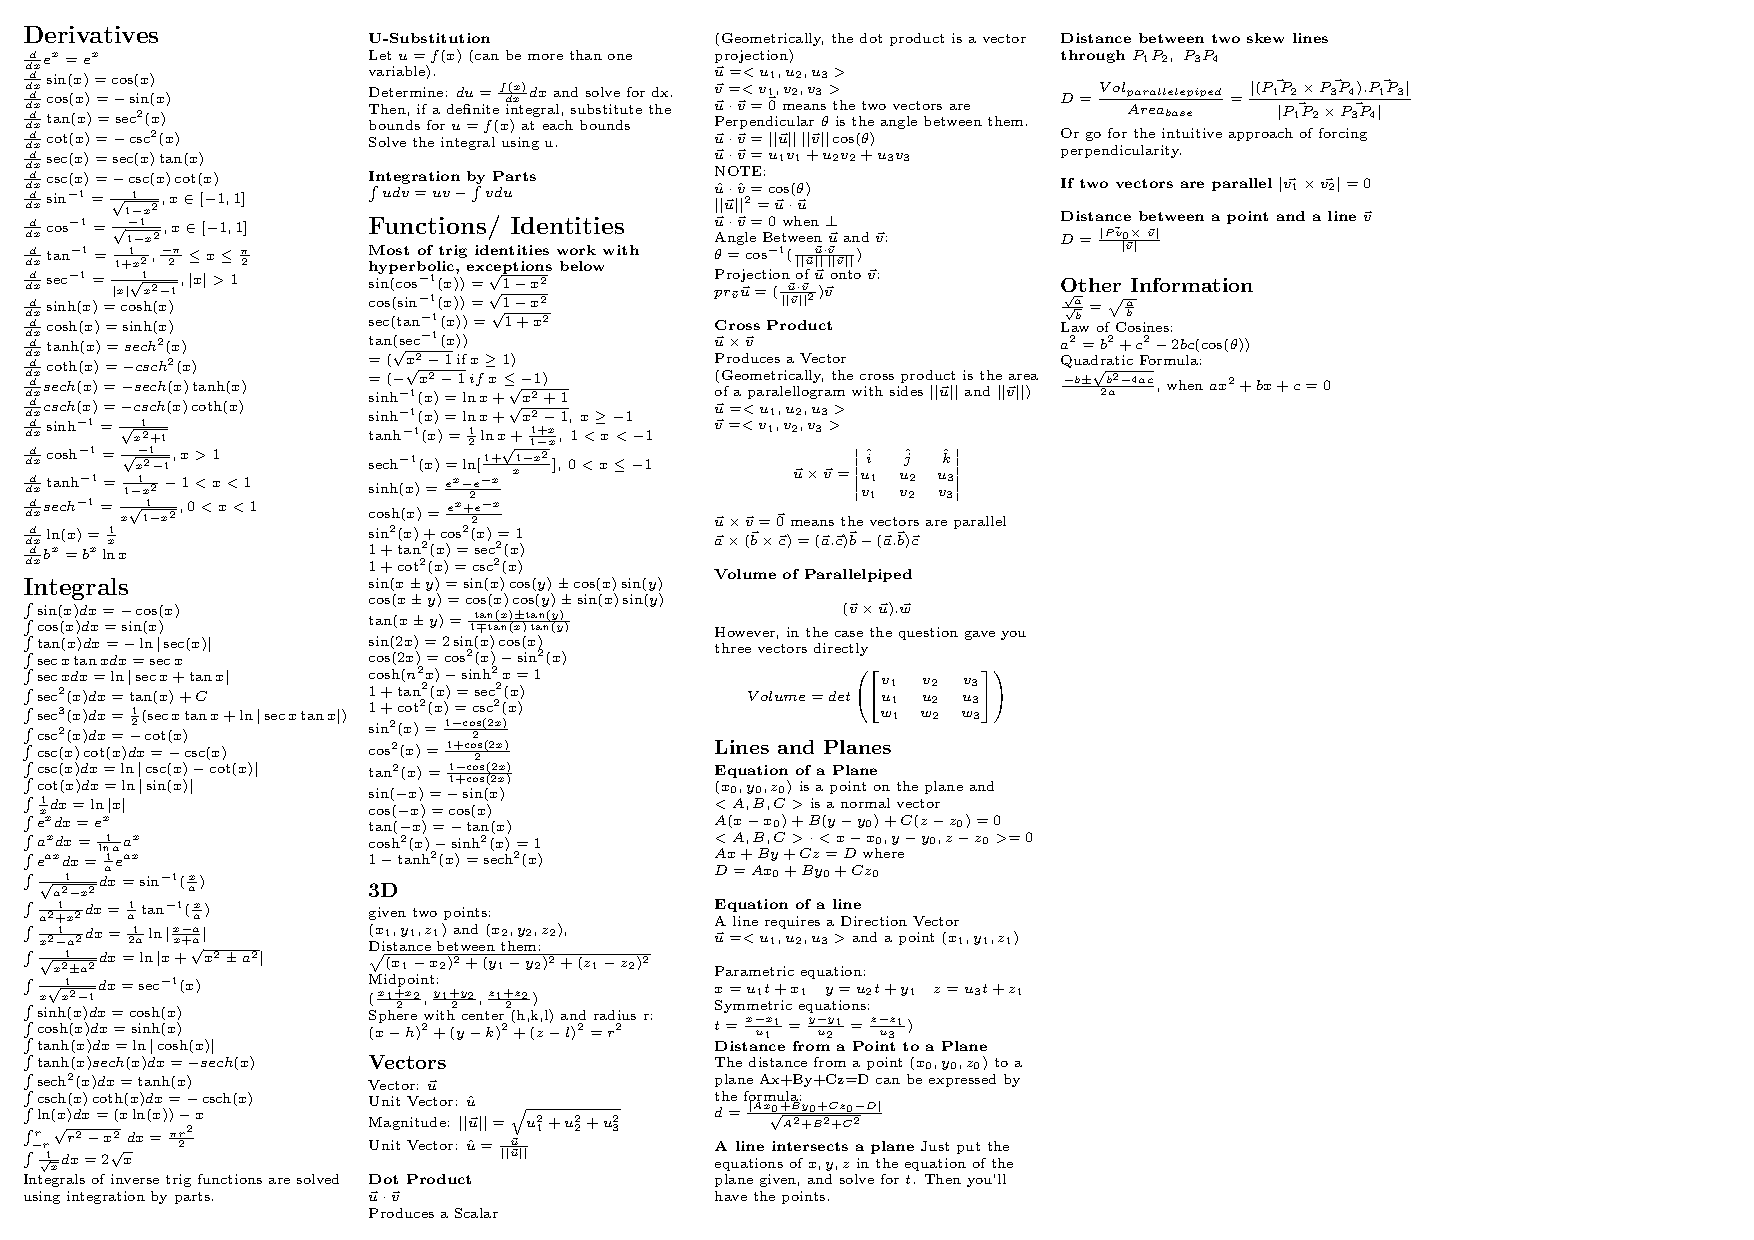
\includepdf[pages=1,fitpaper]{cheatSheet.pdf}

\end{document}
